\documentclass[tikz,border=10pt]{standalone}

\begin{document}
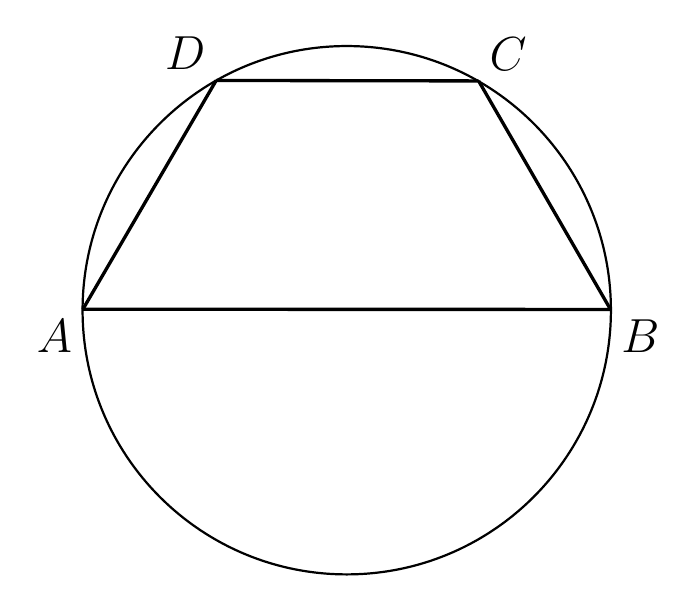
\begin{tikzpicture}[line width=1.2pt, line join=round]
\coordinate (A) at (-3.377,-0.156);
\coordinate (B) at (3.324,-0.158);
\coordinate (C) at (1.649,2.744);
\coordinate (D) at (-1.684,2.750);

  
  
  \coordinate (O) at (-0.026,-0.168);

  
  \draw[line width=0.8pt] (O) circle[radius=3.355];

  
  \draw (A) -- (B);
  \draw (A) -- (D);
  \draw (D) -- (C);
  \draw (C) -- (B);

  
  \node[below left,  font=\fontsize{17.5}{21}\selectfont] at (A) {$A$};
  \node[below right, font=\fontsize{17.5}{21}\selectfont] at (B) {$B$};
  \node[above right, font=\fontsize{17.5}{21}\selectfont] at (C) {$C$};
  \node[above left,  font=\fontsize{17.5}{21}\selectfont] at (D) {$D$};
\end{tikzpicture}
\end{document}